% ============================================================
%  Capítulo 7 — Discussão
% ============================================================
\chapter{DISCUSSÃO}
\label{cap:discussao}

\section{Teto de informação da representação intermediária}
\label{sec:disc-teto}

O resultado mais revelador da Tabela~\ref{tab:bin} não é o melhor F1 absoluto, mas
a resposta quase nula à expansão do espaço de features: passar de bigrams
(4.723~features, F1~=~0,843) para trigrams (50.631~features, F1~=~0,845) representa
um ganho de apenas +0,002 apesar de uma expansão 10,7$\times$ no número de
features. Essa resposta plana indica um teto imposto pela entrada, não pela
capacidade do modelo.

A aritmética do vocabulário explica o fenômeno. O vocabulário da RI contém 136
tokens ativos. Como os bigrams TF-IDF são ordenados (o par
\texttt{load\_global get\_named\_prop} é distinto de
\texttt{get\_named\_prop load\_arg}), o número máximo de bigrams distintos é
$136^2 = 18.496$; o máximo de trigrams é da ordem de
$136^3 \approx 2{,}5 \times 10^6$. O TF-IDF retém, respectivamente, 4.723 e
50.631 features por frequência mínima, ou seja, apenas os n-grams que aparecem
com frequência suficiente no corpus de treinamento. Como o comportamento de
fingerprinting se concentra num subconjunto pequeno de padrões de opcode
(acesso a propriedades, captura de closure, chamadas de API,
try/catch), os bigrams discriminativos estão praticamente exauridos dentro
das 4.723 features retidas. Trigrams adicionam cadeias mais longas, mas estas
apenas reexpressam padrões já capturados por combinações de bigrams; não introduzem
informação nova.

O RF com unigrams (136~features, F1~=~0,834) reforça essa conclusão por outro
ângulo: a frequência de tokens individuais, sem qualquer noção de ordem ou
co-ocorrência, já alcança 0,011 abaixo do melhor modelo. A contribuição marginal de
cada nível de n-gram é decrescente e pequena.

O teto situa-se em aproximadamente \textbf{F1 $\approx$ 0,85} para detecção
cross-engine baseada exclusivamente em bytecodes. Os $\approx$15\% de erro residual
não podem ser fechados com n-grams mais ricos sobre o mesmo vocabulário de 145
tokens. Três fontes de informação ausentes nos bytecodes poderiam reduzir esse
erro:

\begin{enumerate}
\item \textbf{Nomes de funções e contexto de grafo de chamadas.} O modelo atual não
  distingue uma função \texttt{canvasFingerprint} de uma função
  \texttt{renderButton} se ambas produzirem sequências de RI similares. Nomes e
  posição no grafo de chamadas identificam funções orquestradoras que não tocam a
  API diretamente.

\item \textbf{Valores em tempo de execução.} Um mesmo bytecode
  \texttt{GET\_NAMED\_PROP} pode ler \texttt{screen.width} (FP) ou
  \texttt{div.offsetWidth} (layout legítimo). A distinção requer conhecimento do
  valor do receptor, informação ausente no traço estático de bytecodes.

\item \textbf{Vocabulário de opcodes mais fino.} A RI abstrai variantes de opcodes
  que o V8 e o SpiderMonkey distinguem (ex.: \texttt{LdaSmi} vs.\
  \texttt{LdaConstant} $\to$ ambos \texttt{LOAD\_INT}). Preservar essas distinções
  aumentaria a expressividade, ao custo de reduzir a portabilidade entre motores.
\end{enumerate}

\textbf{Features estruturais e contexto de script.} Para testar se o teto poderia
ser elevado sem abandonar a resistência à ofuscação, dois grupos de features
adicionais foram avaliados via ablação (Seções~\ref{sub:estrutural}
e~\ref{sec:oracle}). O primeiro, seis features estruturais locais derivadas
diretamente da sequência de tokens da RI, não produziu ganho mensurável sobre
o baseline de bigrams (F1~=~0,842~vs.~0,843, $\approx{-}0{,}001$), confirmando que as frequências
TF-IDF já codificam implicitamente essas estatísticas. O segundo grupo, contagem
real de funções FP no mesmo script, calculada sobre as 68M linhas com os rótulos
reais do dataset, produziu um salto de +0,075~F1 (F1~=~0,928
vs.~0,853). Esse experimento delimita o \textbf{limite superior oracle}:
o desempenho máximo atingível pela co-ocorrência de script, pressupondo perfeita
rotulagem prévia de todas as funções vizinhas. Como essa condição não se verifica
em produção, F1~=~0,928 não é implantável (ver Seção~\ref{sec:oracle}).

\textbf{Inferência iterativa: F1~=~0,904 sem rótulos oracle.} Para recuperar parte
do intervalo de 0,075 sem vazar rótulos, foi implementada uma estratégia de
inferência iterativa. A primeira passagem classifica todas as 68M funções com o
modelo de densidade e acumula, por script, a contagem absoluta de funções com
probabilidade acima de 0,50 e o logaritmo do tamanho total.
Nenhum rótulo real é consultado. A segunda passagem retreina o LightGBM com essas
três features de contexto (densidade, contagem e logaritmo do tamanho), atingindo
F1~=~0,874. Ciclos adicionais de auto-melhora, expandindo para três contagens em
limiares distintos ($p{>}0{,}30$; $p{>}0{,}50$; $p{>}0{,}70$) e recomputando as
contagens com o modelo da iteração anterior, produzem \textbf{F1~=~0,901} (iter.~2)
e \textbf{F1~=~0,904} (P~=~0,934, R~=~0,876, limiar~=~0,80, iter.~3). A progressão
por iteração é +0,021, +0,027, +0,003, confirmando convergência com retornos
decrescentes. O modelo da
iteração~3 recupera $\approx$68\% do intervalo oracle (0,051 de 0,075) e é o
\textbf{resultado implantável principal} deste trabalho: F1~=~0,904 atingível
sem nenhum rótulo prévio.

A estratégia de contagens em múltiplos limiares captura a forma da
distribuição de probabilidades dentro de cada script: um script com muitas funções
a $p \approx 0{,}4$ (positivos suaves) é qualitativamente diferente de um com
poucas funções a $p{>}0{,}70$ (positivos de alta confiança), mesmo que o número de
funções com $p{>}0{,}5$ seja idêntico. Os split gains das cinco features de
contexto dominam as colunas de importância \emph{no modelo iterativo}, superando
individualmente os bigrams TF-IDF mais informativos nesse mesmo modelo. Nota: os
ganhos do modelo iterativo (escala de unidades a milhar, 1.000 árvores, com
features de contexto que redistribuem o ganho) não são diretamente comparáveis
com os da Tabela~\ref{tab:features-imp}, que apresenta os ganhos do modelo base
de bigrams sem contexto (500 árvores, escala de centenas de milhares).

\textbf{Irredutibilidade do intervalo remanescente.} Uma questão natural é se o
contexto de grafo de chamadas (identificar quais funções orquestradoras invocam
rotinas FP sem tocar a API diretamente) poderia fechar a diferença de 0,024
ainda existente. Para verificar isso empiricamente, os registros de chamadas de API produzidos
pelo script de conteúdo da extensão foram inspecionados. A extensão captura
pilhas de chamadas completas: registros consecutivos com o mesmo par
\texttt{(api, page\_url)} representam quadros sucessivos de uma única cadeia de
chamadas, do invocador direto da API até todos os envolvedores orquestradores.
Entretanto, o pós-processador já consome essa informação integralmente via
propagação de contenção: toda função que apareça em qualquer posição de uma
pilha de chamadas capturada é rotulada como FP, independentemente de ter invocado
a API diretamente. Os rótulos de cadeia de chamadas já estão presentes nos dados de
treinamento; nenhum sinal novo é extraível dos registros de pilha existentes.

A diferença remanescente de 0,024 não reflete ausência de cobertura do grafo de
chamadas. Ela reflete uma classe de sequências de bytecodes genuinamente ambíguas:
funções stub intermediárias corretamente rotuladas como FP por participarem da cadeia
de chamadas, mas cujas sequências de tokens de RI são indistinguíveis de
closures utilitárias comuns (comprimento médio $\approx$96~tokens — acima da
média do corpus de $\approx$65~tokens, pois são funções orquestradoras com
alguma lógica de controle —, fluxo de controle genérico, nenhuma assinatura de opcode específica de API). Nenhuma feature
derivável do dataset existente pode resolver essa ambiguidade. Fechá-la exigiria
informação que bytecodes estáticos não carregam: valores em tempo de execução que
distinguem \texttt{screen.width} de \texttt{div.offsetWidth}, ou nomes de fonte que
identificam \texttt{canvasFingerprint} em vez de \texttt{renderHelper}. Esse
resultado estabelece um teto superior principiado, no nível do dataset, que
profissionais podem usar para avaliar quando abordagens baseadas exclusivamente em
bytecodes são suficientes e quando sinais complementares precisam ser adicionados.

%, , , , , , , , , , , , , , , , , , , --
\section{Necessidade do treinamento conjunto}
\label{sec:disc-conjunto}

A existência de uma RI com vocabulário compartilhado é condição necessária,
mas não suficiente, para a generalização cross-engine. Os experimentos de
transferência zero-shot (Tabela~\ref{tab:zeroshot}) demonstram isso empiricamente:
mesmo com os mesmos 136 tokens de RI em ambos os motores, treinar em Chromium e
testar em Firefox produz F1~=~0,149; a direção inversa produz F1~=~0,180. Ambos os
resultados são próximos de um classificador aleatório calibrado para alta
revocação.

A causa é distribucional. V8 e SpiderMonkey compilam operações JavaScript
semanticamente idênticas em ordens de tokens distintas, como discutido na
Seção~\ref{sec:ir-motivacao}. Um bigram como \texttt{load\_global get\_named\_prop}
é frequente em sequências V8 para o padrão \texttt{navigator.hardwareConcurrency};
o SpiderMonkey pode produzir \texttt{get\_named\_prop load\_arg} para a mesma
operação. Após a tradução para RI, os unigrams são idênticos, mas os
bigrams diferem — a Figura~\ref{fig:zeroshot-vs-conjunto} ilustra essa
divergência nas distribuições de bigramas por motor. Um classificador TF-IDF
treinado exclusivamente em sequências V8 aprende limiares de decisão moldados
pela distribuição de bigrams do V8; esses limiares não transferem para a
distribuição estruturalmente diferente do SpiderMonkey.

\begin{figure}[htb]
\centering
\caption{Distribuições de bigramas de RI por motor: divergência entre V8 e SpiderMonkey}
\label{fig:zeroshot-vs-conjunto}
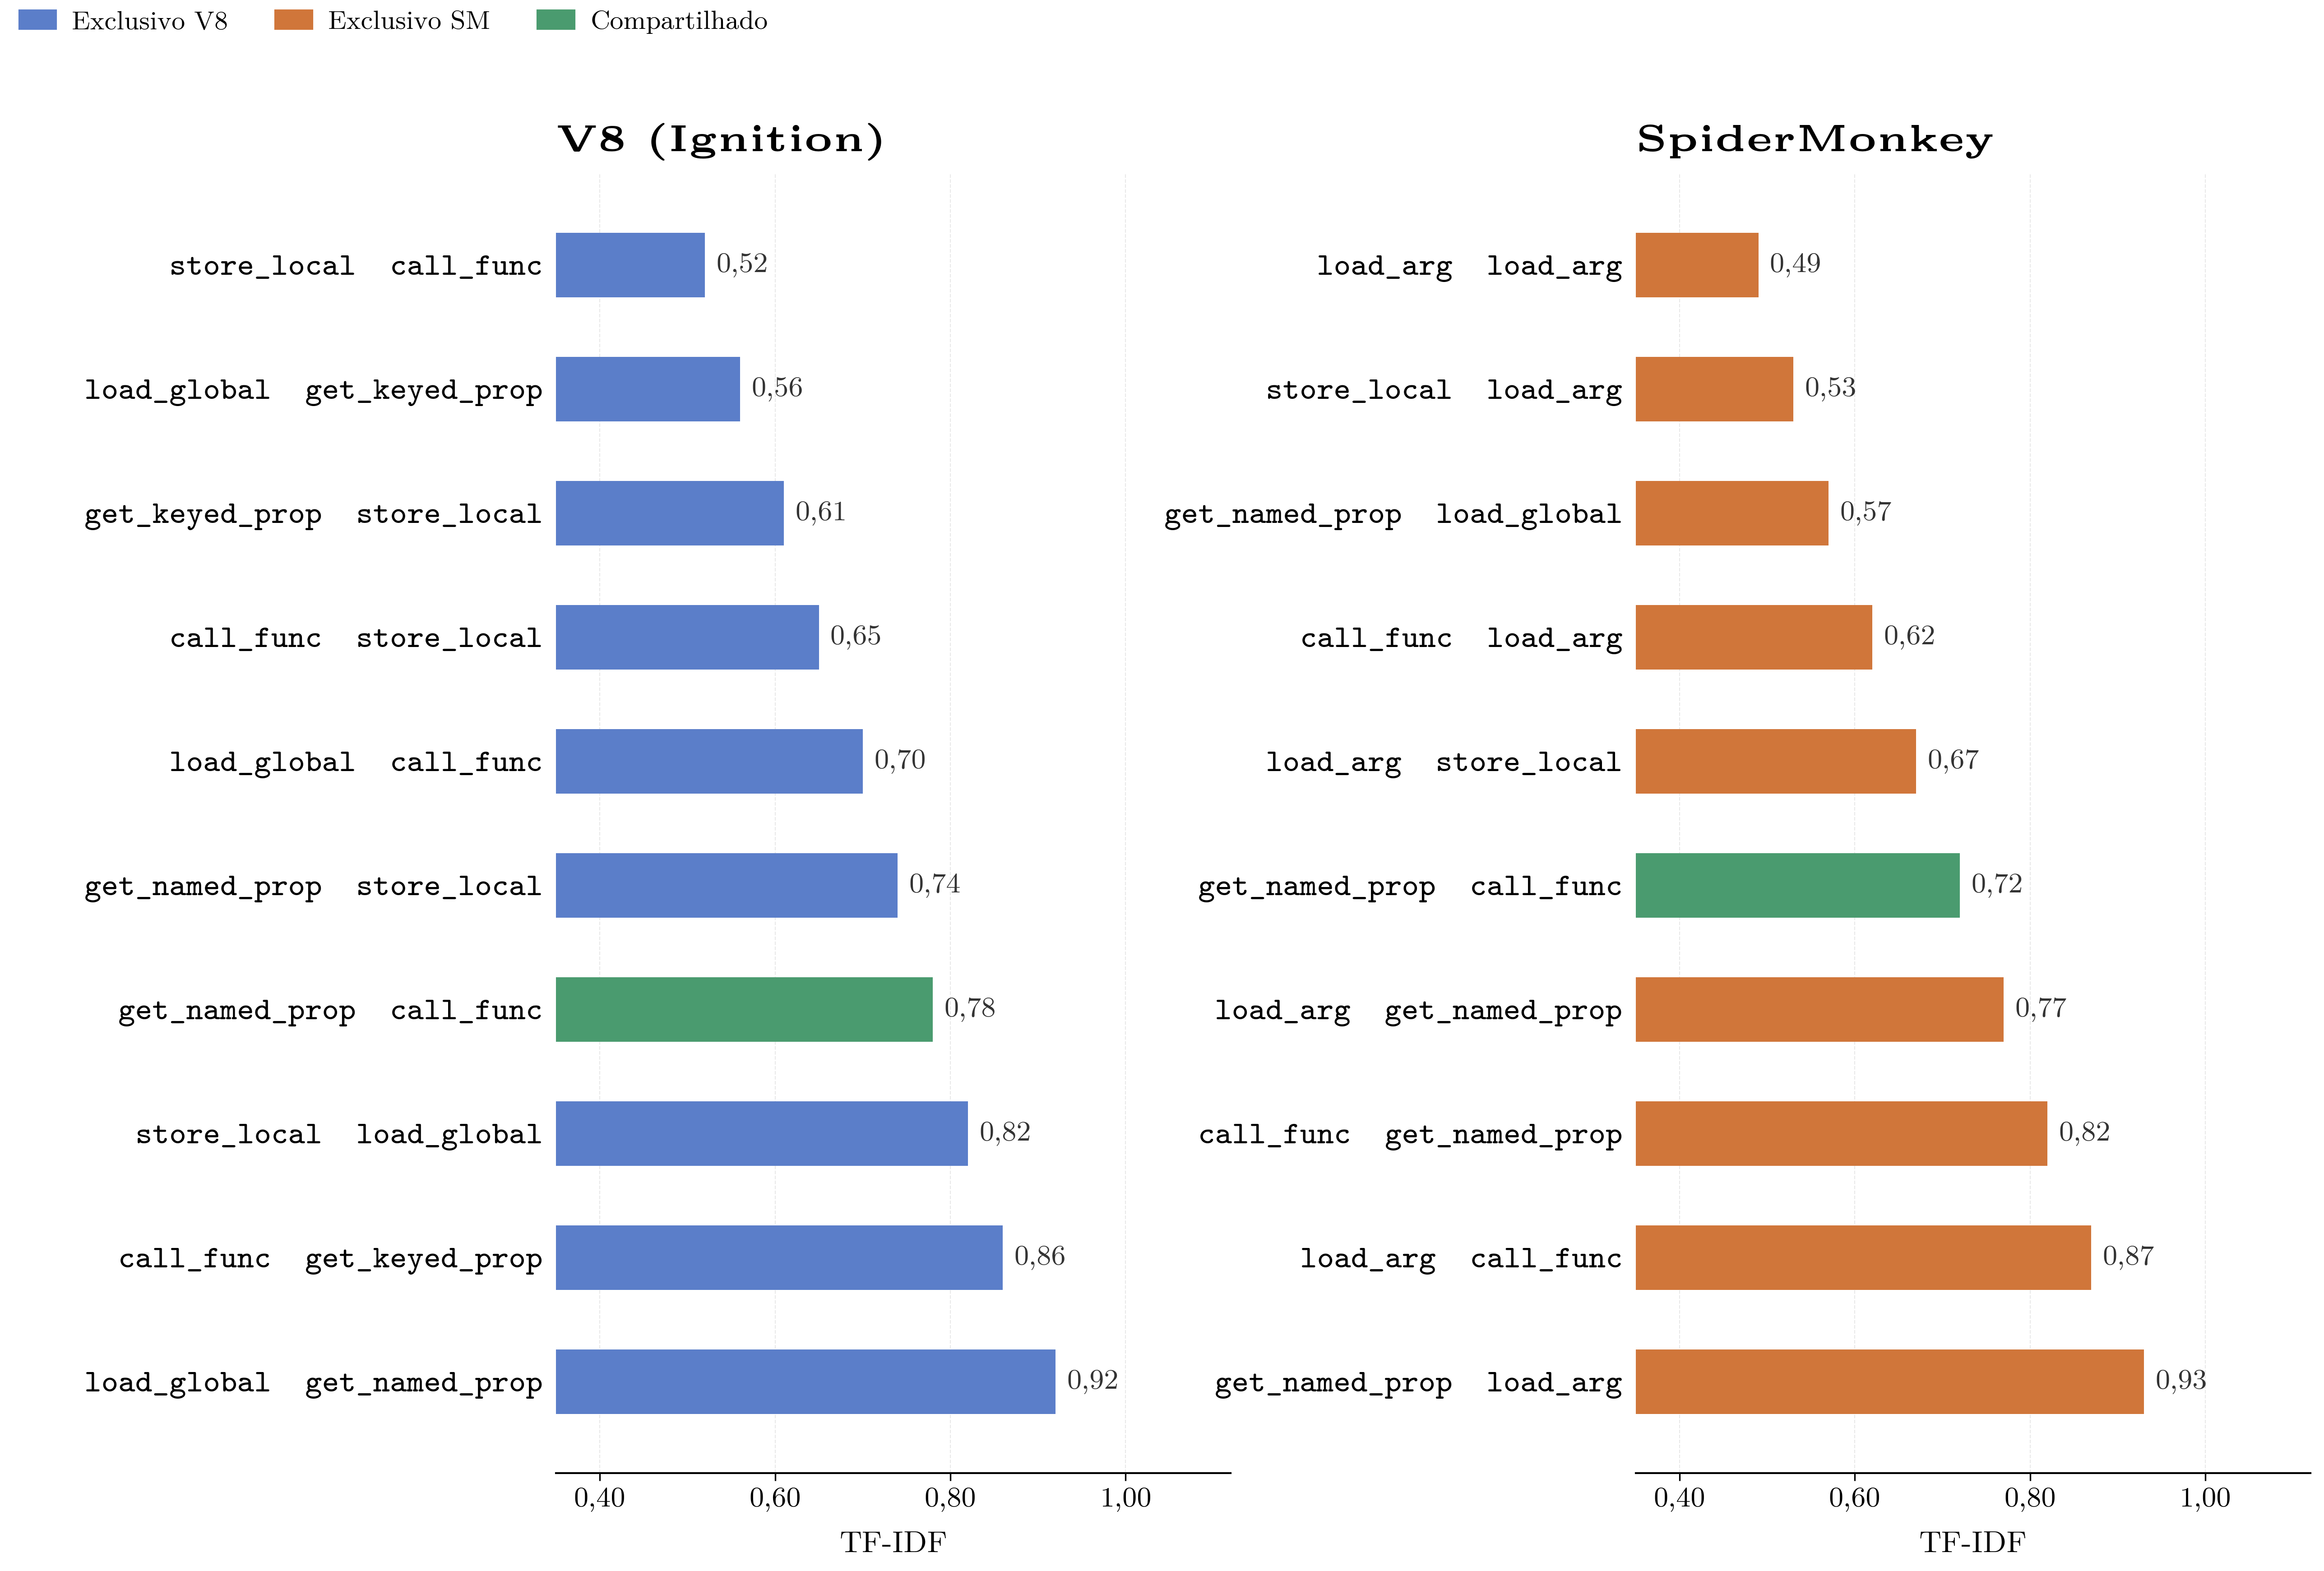
\includegraphics[width=0.88\linewidth]{fig_zeroshot_vs_joint}
\fonte{Elaborada pelo autor.}
\end{figure}

O treinamento conjunto resolve o problema ao expor o modelo às duas distribuições
simultaneamente durante o treinamento. O vocabulário compartilhado da RI garante
que os mesmos nomes de features indexem frequências comparáveis em ambos os
corpora; o modelo aprende uma superfície de decisão que generaliza sobre as duas
distribuições. O resultado (Tabela~\ref{tab:conjunto}) é um único conjunto de pesos
que atinge F1~=~0,877 no Chromium e F1~=~0,847 no Firefox com o modelo de bigrams
básico, ou F1~=~0,903 e F1~=~0,904 quando aumentado pelas features de contexto
iterativo (Tabela~\ref{tab:conjunto-iter}).

A implicação para extensibilidade é direta. Adicionar suporte a um terceiro motor
por exemplo, JavaScriptCore (Safari), exigiria: (i) instrumentar o
JavaScriptCore para emitir bytecodes; (ii) estender o dicionário de equivalência
com mapeamentos para os opcodes do novo motor, preservando os 145 tokens do dicionário de equivalência (136 ativos no TF-IDF);
e (iii) retreinar o modelo conjunto incluindo dados do terceiro motor. Não seria
necessário criar um modelo separado nem modificar os classificadores dos motores
existentes.

%, , , , , , , , , , , , , , , , , , , --
\section{Custo da independência de motor: comparação com ByteDefender}
\label{sec:disc-bytedefender}

O ByteDefender \cite{nikkhahbahrami2025} reportou F1~$\approx$~0,950 usando
bytecodes brutos do V8 em um corpus de motor único. Este trabalho atinge
F1~=~0,904 usando a RI cross-engine num corpus misto V8 + SpiderMonkey. A
diferença de \textbf{$\approx$5 pontos de F1} existe, mas os dois sistemas não
resolvem o mesmo problema: a tarefa deste trabalho é estritamente mais difícil
em três eixos.

\textbf{Funções anônimas e lambda incluídas.} O ByteDefender operou sobre funções
nomeadas, diretamente identificáveis nos metadados de bytecodes. Este trabalho
rastreia funções anônimas injetando IDs únicos em tempo de compilação (injeção de
\texttt{displayName} no SpiderMonkey; correspondência por posição no Chromium),
capturando funções cujos bytecodes não carregam nenhum sinal derivado do nome.
Funções anônimas representam uma parcela significativa do dataset; suas sequências
de bytecodes são genericamente indistinguíveis de closures utilitárias
comuns.

\textbf{Sete categorias de fingerprinting, não quatro.} O ByteDefender
cobriu canvas, fonte, áudio e WebRTC. Este trabalho inclui adicionalmente WebGL,
tela e navigator, categorias que tendem a aparecer em funções menores e
estruturalmente mais genéricas, aumentando a proporção de positivos difíceis no
dataset.

\textbf{Nenhum metadado como feature.} Apenas sequências de tokens de RI são
usadas, sem nomes de funções, URLs de script ou qualquer identificador de
contexto. O conjunto de features do ByteDefender não é completamente especificado
no artigo, mas nomes de funções como \texttt{getCanvasFingerprint} ou
\texttt{collectAudioContext} são metadados trivialmente discriminativos que
inflariam o F1 substancialmente se incluídos. A exclusão deliberada desses sinais
produz um classificador intrinsecamente robusto à renomeação de funções e à
minificação, condições comuns em bundles de produção.

Diante dessas três diferenças, a diferença de $\approx$5 pontos deve ser
interpretada como o \textbf{custo combinado da independência de motor, da inclusão
de funções anônimas, de um espaço de rótulos mais amplo e de um espaço de features
sem metadados}, não como deficiência da abordagem cross-engine.

Três fatores técnicos também contribuem para a diferença.

\textbf{Perda por abstração da RI.} O conjunto de opcodes brutos do V8 contém 198
instruções distintas mapeadas no dicionário; a RI as colapsa em 145 tokens (136 ativos
no TF-IDF após descarte de tokens raros e dos dois nunca observados no corpus).
Cada fusão descarta distinções que o modelo de motor único do ByteDefender pôde
explorar. A cobertura de 99,82\% significa que quase nenhum token é perdido, mas
muitos são agrupados, e esses agrupamentos apagam distinções discriminativas no
contexto de motor único.

\textbf{Ruído distribucional do corpus conjunto.} Para a mesma construção
JavaScript, V8 e SpiderMonkey geram padrões de n-grams distintos sob a mesma RI.
O modelo conjunto deve aprender uma superfície de decisão que satisfaça
simultaneamente ambas as distribuições, um problema estritamente mais difícil do
que ajustar uma única distribuição.

\textbf{Composição do dataset.} O dataset deste trabalho apresenta taxa de
positivos de 0,055\% nos 10.000 sites mais populares da lista Tranco, com 37.644
funções FP em 68 milhões de funções totais. A composição do dataset do ByteDefender
seleção de sites, profundidade de crawl e taxa de positivos, não foi
divulgada publicamente.

Apesar do gap, a perspectiva prática favorece a portabilidade. Com a inferência
iterativa (iter.~3, Seção~\ref{sec:iterativo}), este trabalho atinge
F1~=~0,904 no conjunto combinado V8 + SpiderMonkey sem retreinamento por motor.
Com contexto iterativo, o modelo conjunto atinge F1~=~0,903 no Chromium e
F1~=~0,904 no Firefox em avaliação por motor separada, a $\approx$0,047 do
ByteDefender, sem retreinamento por motor. A
Tabela~\ref{tab:bytedefender} sintetiza o posicionamento comparativo.

\begin{table}[htb]
\centering
\caption{Comparação com ByteDefender}
\label{tab:bytedefender}
\begin{tabularx}{\linewidth}{l>{\raggedright\arraybackslash}X>{\raggedright\arraybackslash}X}
\toprule
\textbf{Propriedade} & \textbf{ByteDefender} & \textbf{Este trabalho} \\
\midrule
Motores suportados                & V8 (Chromium)   & V8 + SpiderMonkey \\
Funções anônimas/lambda           & Não             & Sim (ID injetado em tempo de compilação) \\
Categorias de fingerprinting      & 4               & 7 \\
Features utilizadas               & Bytecodes brutos V8 & RI cross-engine (145 tokens, 136 ativos) \\
Melhor F1 binário (implantável)   & $\approx$0,950  & \textbf{0,904} (LightGBM + contexto iterativo, iter.\ 3) \\
Melhor F1 binário (limite oracle) & $\approx$0,950  & \textbf{0,928} (LightGBM + contexto de script real) \\
F1 no Chromium$\star$              & $\approx$0,950  & \textbf{0,903} (modelo conjunto + contexto iterativo) \\
F1 no Firefox (modelo conjunto)   & ---             & \textbf{0,904} (com contexto iterativo) \\
Retreinamento para novo motor     & Obrigatório     & Não necessário \\
Tamanho do modelo recomendado     & -               & 7,1~MB (LightGBM + TF-IDF) \\
\bottomrule
\end{tabularx}
{\footnotesize $\star$ByteDefender opera exclusivamente no Chromium (motor único, sem modelo conjunto);
o valor $\approx$0,950 é do modelo de motor único. O valor 0,903 deste trabalho é do modelo conjunto V8+SM.}

\fonte{Elaborada pelo autor.}
\end{table}

Para um detector implantado num ecossistema heterogêneo de navegadores, a
eliminação do retreinamento por motor representa uma redução substancial de esforço
de engenharia. O custo de $\approx$5 pontos de F1 é o preço mensurável dessa
portabilidade, considerando uma tarefa de classificação estritamente mais difícil.

%, , , , , , , , , , , , , , , , , , , --
\section{Limites do multilabel para rótulos raros}
\label{sec:disc-raro}

A tarefa multilabel expõe uma dificuldade que a tarefa binária obscurece: as sete
categorias de fingerprinting não têm suporte comparável no dataset, e a
assimetria entre a mais comum (Tela: 24.939 funções FP) e as mais raras (WebRTC:
180; Fonte: 208) abrange aproximadamente duas ordens de magnitude (razão $\approx$138:1). Esse nível de escassez interage
de formas distintas com cada família de modelos. O LightGBM com balanceamento automático de classes colapsa nos rótulos raros:
o classificador WebRTC prediz positivo para quase toda função testada, obtendo
P~=~0,0007 e F1~=~0,001 --- a heurística foi projetada para o regime de
desbalanceamento binário simples e sobre-corrige com apenas 39 positivos contra
$\approx$105.123 negativos no conjunto de teste (105.162 instâncias totais menos
39 positivos WebRTC).
O Transformer com Focal Loss também não converge para os rótulos raros dentro
do budget de treinamento testado, com apenas 39 positivos de teste por rótulo raro
(WebRTC e Fonte; os conjuntos de treino correspondentes têm $\approx$144 e
$\approx$166 positivos respectivamente, ainda insuficientes para os rótulos raros).

O RF com \texttt{balanced\_subsample} tolera melhor a escassez porque o balanceamento
opera no nível da árvore individual: cada árvore vê uma visão balanceada de seus
dados de bootstrap, mas o ensemble não adota um limiar de decisão extremo. Os
classificadores WebRTC e Fonte produzem F1~=~0,201 e F1~=~0,345, baixos, mas não
degenerados. Para os rótulos bem suportados (Tela, WebGL, Navigator e Canvas), todos
os três modelos produzem F1 acima de 0,68, confirmando que os bytecodes da RI
carregam sinal multilabel genuíno quando o suporte é adequado. O caminho mais direto
para melhorar WebRTC e Fonte é a coleta direcionada de sites conhecidos por usar
esses vetores, não melhorias no modelo. Os resultados completos estão na
Tabela~\ref{tab:multilabel}.

%, , , , , , , , , , , , , , , , , , , --
\section{Implantabilidade prática}
\label{sec:disc-implantacao}

Os resultados de latência (Tabela~\ref{tab:inferencia}) estabelecem que a detecção
cross-engine por bytecodes é praticável sem hardware especializado. Com lote de
1.000 funções, o modelo LightGBM de bigrams classifica a \textbf{44~µs por função}
em CPU de propósito geral. Uma página web típica aciona algumas centenas de funções
JavaScript durante o carregamento; a vazão de $\approx$22.700~funções/segundo
significa que o traço de bytecodes de uma página completa seria classificado em
\textbf{menos de 15~ms}, imperceptível ao usuário.

O tamanho do artefato de implantação é compacto: o modelo LightGBM de bigrams
ocupa 7,0~MB serializado, mais 140~KB para o vetorizador TF-IDF, total de
$\approx$7,1~MB. Esse footprint é adequado para inclusão em extensões de
navegador, proxies de rede ou pipelines de análise pós-crawl.

Três cenários de implantação são viáveis com os artefatos produzidos:

\textbf{Extensão de navegador em tempo real.} O content script já
instrumentado (Capítulo~\ref{cap:arquitetura}) pode ser estendido para enviar
bytecodes capturados para um serviço local ou embutir o modelo TF-IDF + LightGBM
diretamente em WebAssembly. A latência de 44~µs por função a lotes de 1.000 é
compatível com análise em tempo real durante o carregamento da página.

\textbf{Proxy de rede ou gateway de segurança.} Um proxy que intercepte respostas
JavaScript pode executar o modelo offline sobre bytecodes pré-compilados,
sinalizando scripts com alta densidade de funções FP detectadas antes de repassá-los
ao cliente.

\textbf{Auditoria de crawl em escala.} O pipeline completo demonstrou
viabilidade em escala de 68 milhões de funções; o processamento pós-crawl é
o caso de uso de menor latência exigida e maior throughput disponível.

As limitações operacionais conhecidas do sistema são as seguintes. \textbf{Web
Workers} não são cobertos pela extensão de captura: APIs de fingerprinting
invocadas em Workers (contexto isolado) não são registradas. \textbf{Funções carregadas de forma lazy} só aparecem
nos logs de bytecodes se o navegador as compilar durante a visita; funções em
pacotes de rota que não são ativados pelo crawler são invisíveis ao pipeline.
\textbf{\texttt{eval} e \texttt{new Function}} recebem um \texttt{injected\_id}
baseado na posição da chamada \texttt{eval}, não no código gerado, o que pode
causar colisões em frameworks que geram código dinamicamente. Nenhuma dessas
limitações é específica da abordagem cross-engine proposta; todas afetam igualmente
qualquer sistema baseado em instrumentação de bytecodes.
